\documentclass{aip-cp}

\usepackage[numbers]{natbib}
\usepackage{rotating}
\usepackage{graphicx}
\usepackage{caption}
\def\g12{\emph{g12}}
\newcommand{\abbr}[1]{\textsc{\texttt{#1}}}
% Document starts
\begin{document}

% Title portion
\title{Light Meson Decays from Photon-Induced Reactions with CLAS}

\author[aff1]{Michael C. Kunkel\corref{cor1}}
\author[]{for the CLAS Collaboration }
\affil[aff1]{Forschungszentrum J\"ulich, J\"ulich (Germany)}
\corresp[cor1]{m.kunkel@fz-juelich.de}

\maketitle

\begin{abstract}
Photoproduction of the $\pi^0$ meson was studied using the \textsc{\texttt{CLAS}} detector at Thomas Jefferson National Accelerator Facility using tagged incident beam energies spanning the range $E_{\gamma}=$~1.1~GeV~-~5.45~GeV. The measurement is performed on a liquid hydrogen target in the reaction $\gamma p\to pe^+e^-(\gamma)$. The final state of the reaction is the sum of two subprocesses for $\pi^0$ decay, the Dalitz decay mode of $\pi^0\to e^+e^-\gamma$ and conversion mode where one photon from $\pi^0\to \gamma\gamma$ decay is converted into a $e^+e^-$ pair. This specific final state reaction avoided limitations caused by single prompt track triggering and allowed a kinematic range extension to the world data on $\pi^0$ photoproduction to a domain never systematically measured before.

We report the measurement of the $\pi^0$ differential cross-sections $\frac{d\sigma}{d\Omega}$ and $\frac{d\sigma}{dt}$. The angular distributions agree well with the SAID parametrization for incident beam energies below 3~GeV, while an interpretation of the data for incident beam energies greater than 3~GeV is currently being developed. Included in the report will be a discussion of the future wide angle, exclusive photoproduction of $\pi^0$ experiment that will be performed in Hall C.
\end{abstract}

% Head 1
\section{INTRODUCTION}
In hadron physics, photoproduction of single pion is essential to understand the photon-nucleon vertex. At low energies, the photon-nucleon coupling establishes excited nucleon resonances which has been at the forefront of physics ''missing resonances'' search. At high energies single pion photoproduction can be used to test predictions of Regge theory, in which recent calculations~\cite{JPAC} have shown to describe the presented data well. Furthermore, these measurements have shown that the differential cross section for single pion photoproduction at fixed c.m. angles, $\theta_{c.m.}$, of $70^{\circ}$, $90^{\circ}$and$110^{\circ}$ seem to scale as $\frac{d\sigma}{dt} \sim s^{2-n}f(\theta_{c.m.})$, where $s$ and $t$ are the Mandelstam variables and $n$ is the total number of interacting elementary fields in the initial and final state of the reaction. This is predicted by the constituent counting rule~\cite{scaling1,scaling2} and exclusive measurements in $pp$ and  $\bar{p}p$ elastic scattering~\cite{scalingexp5, scalingexp7}, meson-baryon $M p$ reactions~\cite{scalingexp7}, and photoproduction $\gamma N$~\cite{scalingexp2, scalingexp3, scalingexp4, scalingexp6, scalingexp8, scalingexp9, scalingexp10, scalingexp11}  agree well with this rule . The following proceeding detailed the CLAS g12 experiment, the extraction of single neutral pion photoproduction from data, the differential cross-sections through the entire beam energy range of the g12 experiment, a comparison of the differential cross-section with existing world data, as well as the comparison of the data to the model given in~\cite{JPAC}, comparison to the constituent counting rule. Also presented will be an overview of a future measurement to be taken at Hall C to extended the measurement of neutral pion photoproduction at higher photon energies.
\section{CLAS}
The \textsc{\texttt{CLAS}} detector, shown in Fig.~\ref{fig:clas}, is assembled of four types of detectors, five detectors total,  that are arranged in an onion like pattern (around the beam line) covering $\sim 3\pi$ with a diameter of 8~m. Each layer is segmented such that there are six segments around $\phi$ (angle about the beam line), called sectors, each with a polar coverage, $\theta$ (angle from beam line), of approximately $\frac{3}{4}\pi$~radians. Each sector consists of a scintillator start counter (\textsc{\texttt{ST}}), three layers of drift chambers (\textsc{\texttt{DC}}), a layer of scintillator ``time-of-flight'' counters (\textsc{\texttt{TOF}}), a gas Cherenkov counter (\textsc{\texttt{CC}}) and an electromagnetic calorimeter (\textsc{\texttt{EC}}). There is a toroidal magnetic field generated by six superconducting coils that divide the sectors. The direction of the toroidal field is azimuthal, $\phi$ (angle about the beam line), such that the charged particles conserve their azimuthal angle along their trajectory, except near the coils. The magnetic field geometry guides the particles which allows for a simplified reconstruction algorithm to determine the particles' momenta.
\begin{figure}[h]
	\centerline{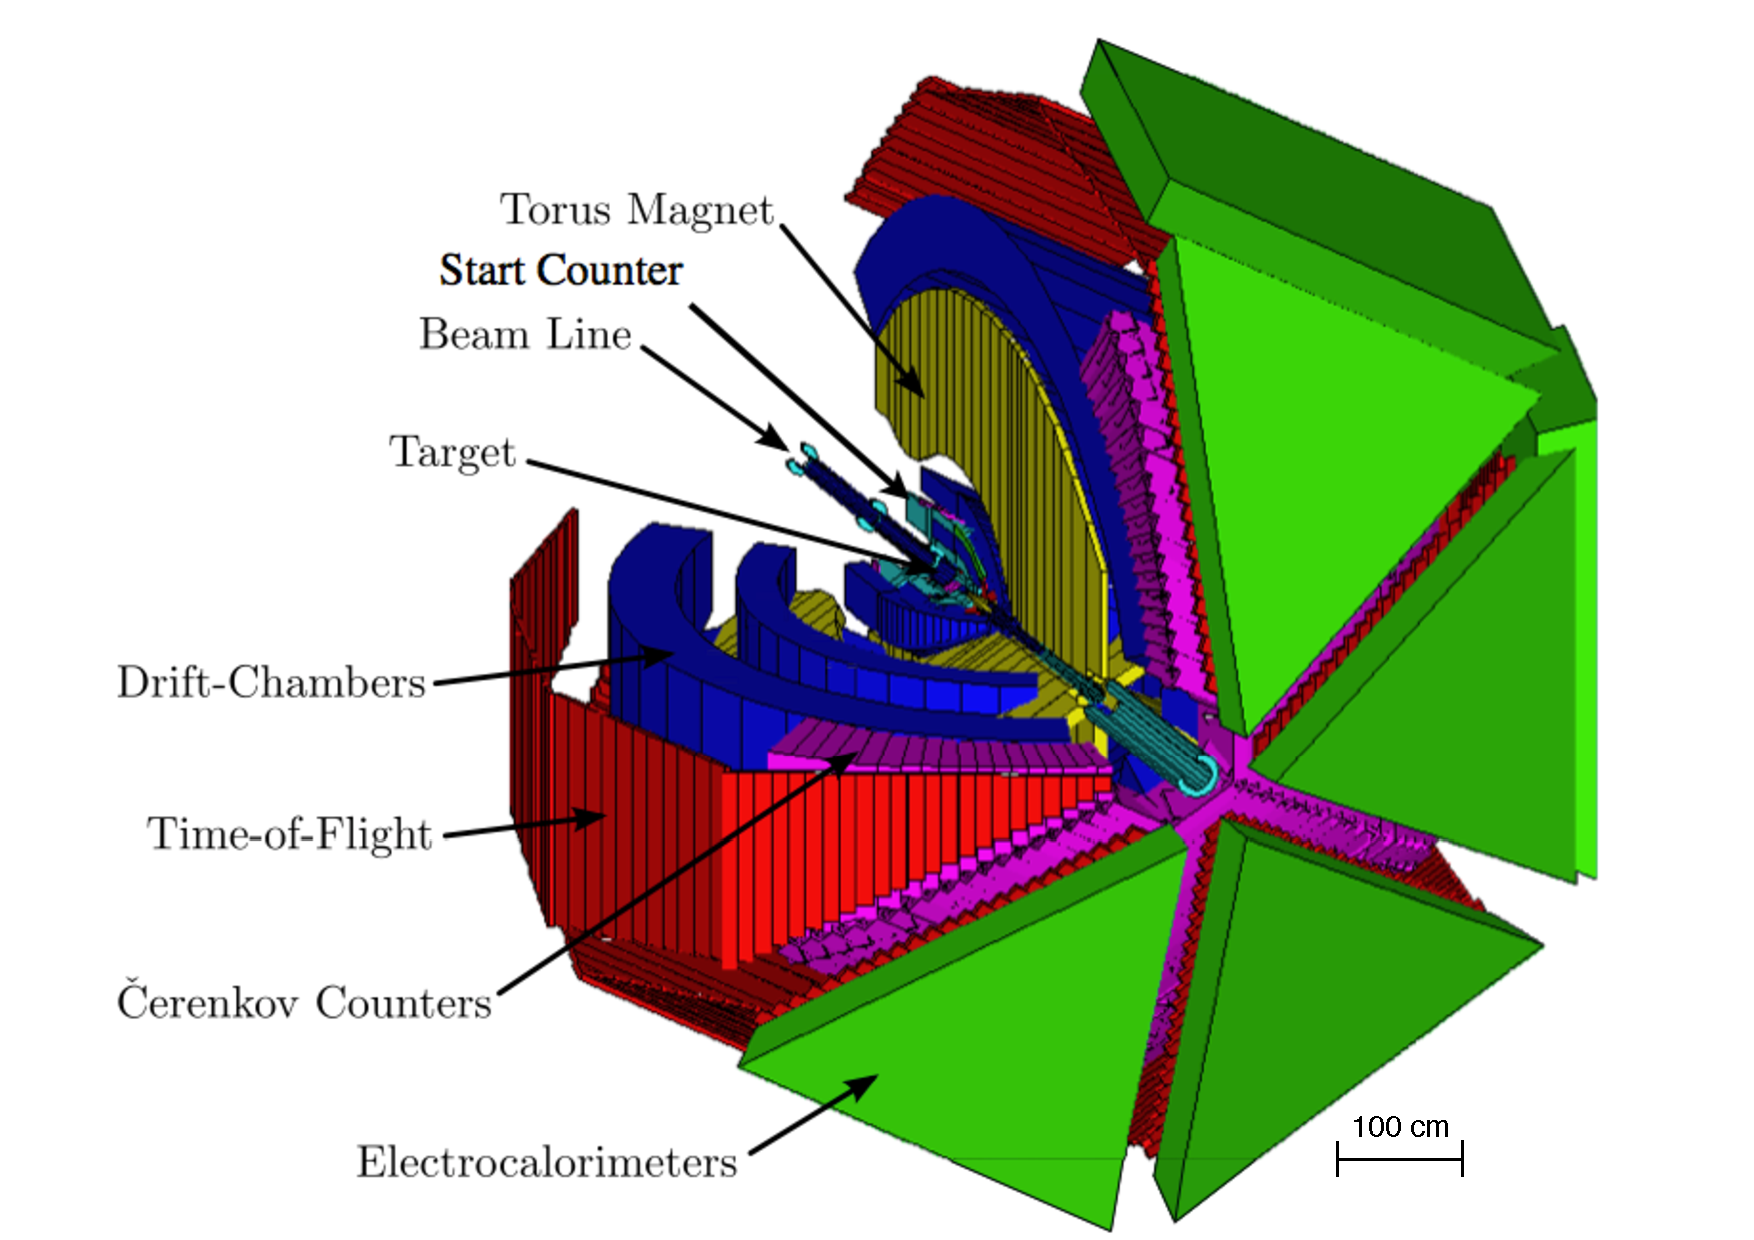
\includegraphics[width=175 pt]{figures/clas_schematicIII.pdf}}
	\caption{The CEBAF Large Acceptance Spectrometer (\textsc{\texttt{CLAS}}) }
	\label{fig:clas}
\end{figure}
\section{The g12 Experiment}
The \g12 experiment is a photoproduction experiment, it ran during March - June 2008 with a total of 44 days of good beam time. It collected over 128~TB of raw data that consisted of $26\cdot 10^9$ events, with an integrated luminosity of 68~pb$^{-1}$. The photon beam was produced by impinging a $5.715$~GeV electron beam, at 65nA, on a Au radiator of $10^{-4}$ radiation length. Photons in the energy range from 20\% to 95\% of the electron beam
energy were tagged, resulting in a photon beam energy range of 1.1-5.5~GeV. This photon beam was then collimated before being introduced onto a $\ell H_2$ target 40~cm in length along the z-direction and 2~cm radius. The placement of the target was 90~cm upstream from \abbr{CLAS} center (toward Au radiator), this increased the acceptance of particles in the forward direction. During the runtime of \g12, the Cherenkov detectors were filled with perfluorobutane ($\mathrm{C_4F_{10}}$) allowing for electron/positron detection. The experiment had a dedicated trigger, amongst 9 other triggers, that consisted of \abbr{CC} and \abbr{EC} coincidence hits for the entire beam energy range. With proper cuts on the \abbr{CC} and \abbr{EC} a $\pi/e$ rejection of $10^6$ for $e^{\pm}$ pairs was established.
\subsection{Particle Selection}
Particle selection consisted of all beam photons that were within 1.002~ns timing coincidence of the event, 1 proton and 2 oppositely charged tracks that were not the proton. This selection is appropriate for identifying the $\pi^0 \to e^+e^-\gamma$ decay because the mass of the $\pi^0$ is less than that of $\pi^{\pm}$, meaning $\pi^0$ cannot decay into $\pi^{+}\pi^{-}$.
\subsection{Kinematic Cuts}
\begin{figure}[h!]
	\centering
	\begin{minipage}{.50\textwidth}
		\centering
		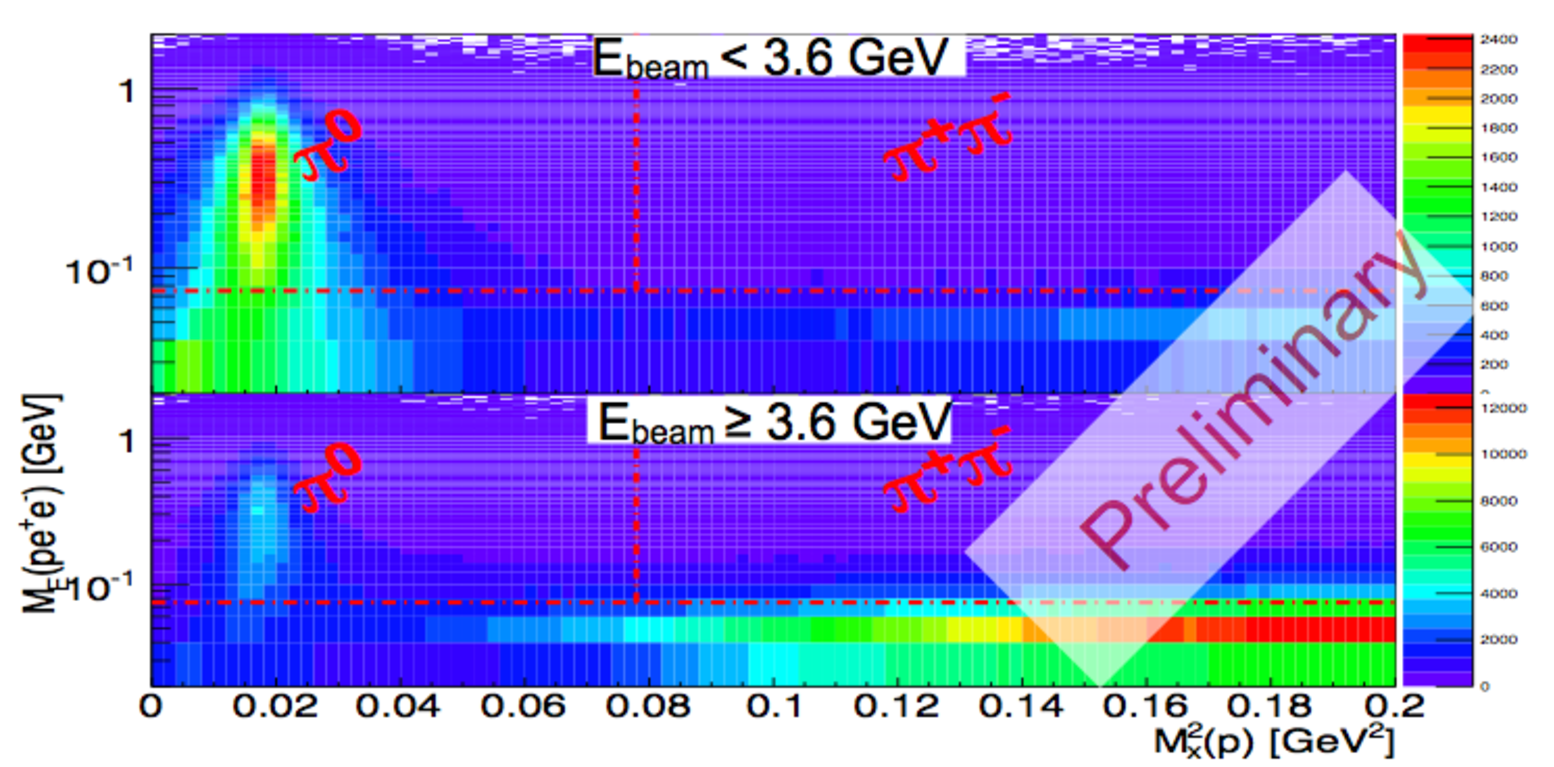
\includegraphics[width=225 pt, height = 150 pt]{figures/pi0_ME_vs_Mx.pdf}
		\caption{}{}
		\label{fig:Mx_ME}
	\end{minipage}%
	\centering
	\begin{minipage}{.50\textwidth}
		\centering
		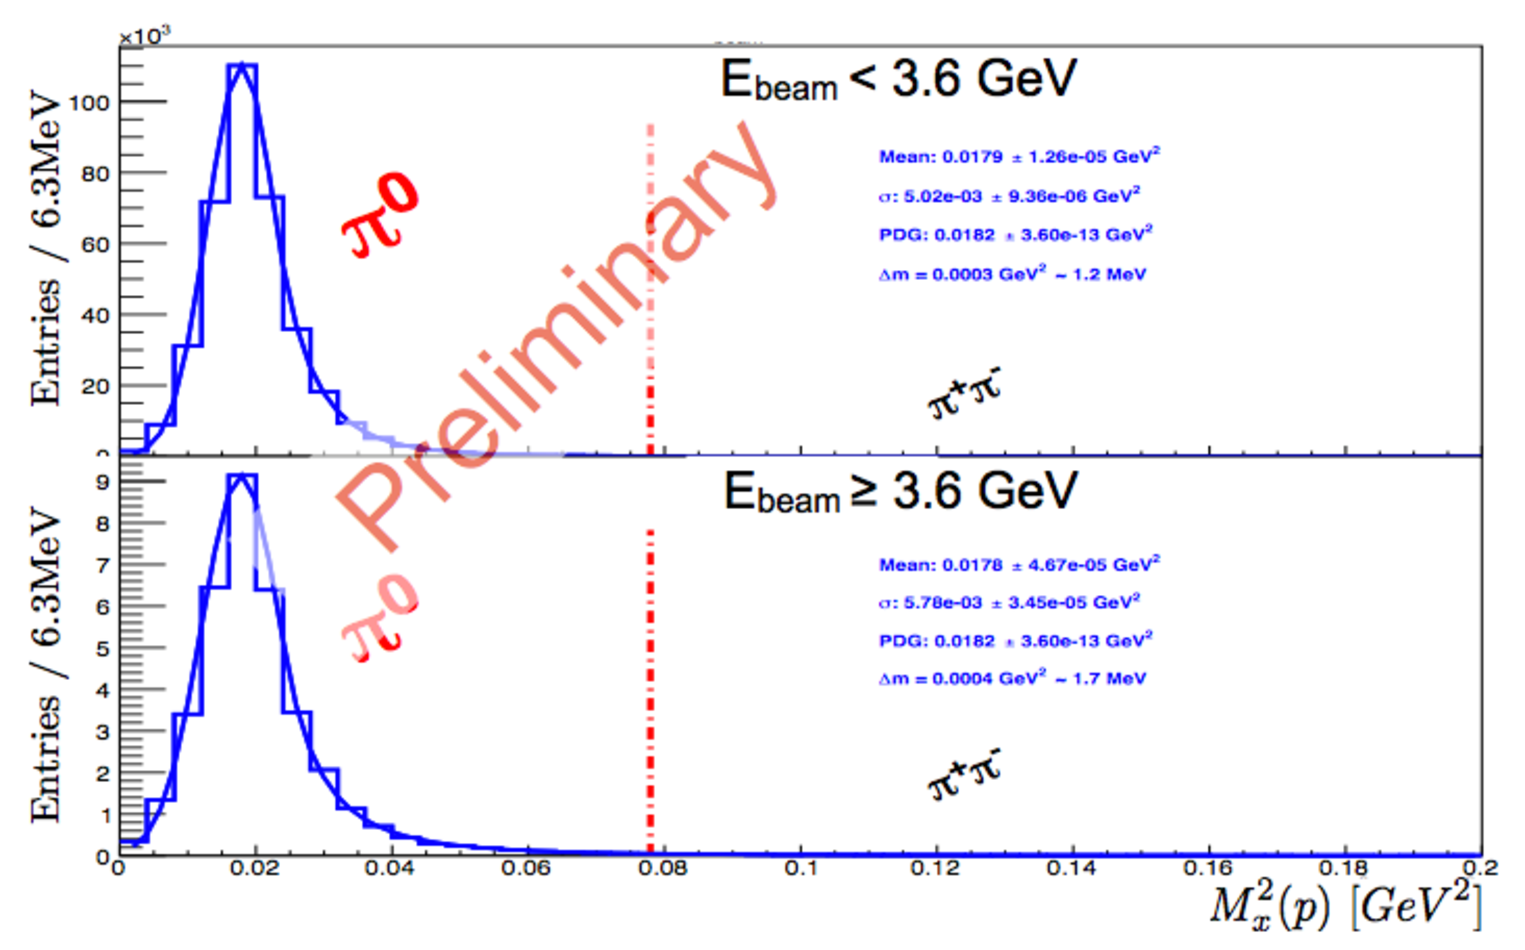
\includegraphics[width=225 pt, height = 150 pt]{figures/pi0_spectrum.pdf}
		%\caption{figure in here}{box diagram}
		\caption{Left: $M_x^2 (p)$ vs. $M_E(pe^+e^-)$. The horizontal red dashed-dotted line depicts the 75 MeV cut used in this analysis. The vertical red dashed-dotted line depicts the boundary of single $\pi^0$ to $\pi^{+}\pi^{-}$ production. Right: Final $M_x^2(p)$ data used in analysis. The horizontal red dashed-dotted line depicts the threshold of $\pi^{+}\pi^{-}$ production.}{}
		\label{fig:Mxp}
	\end{minipage}
\end{figure}
\section{Comparison to Existing Data}
\begin{figure}[h!]
	\centering
	\begin{minipage}{.50\textwidth}
		\centering
		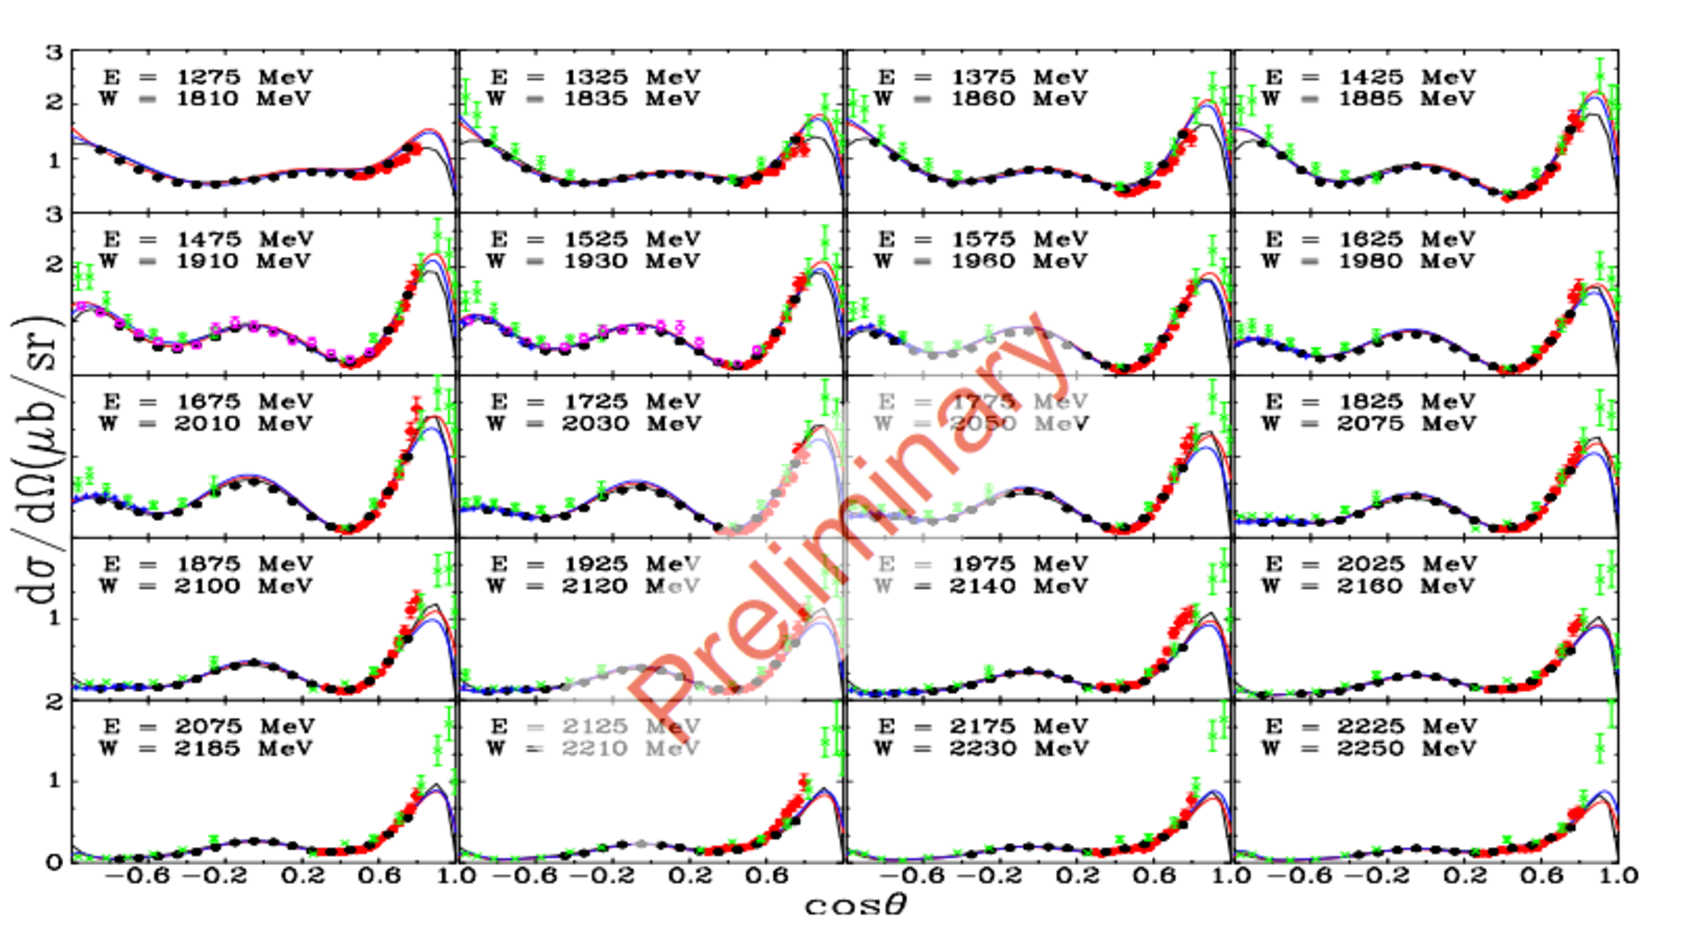
\includegraphics[width=225 pt, height = 160 pt]{figures/pi0_xsectionI.pdf}
		\caption{}{}
		\label{fig:pi0I}
	\end{minipage}%
	\centering
	\begin{minipage}{.50\textwidth}
		\centering
		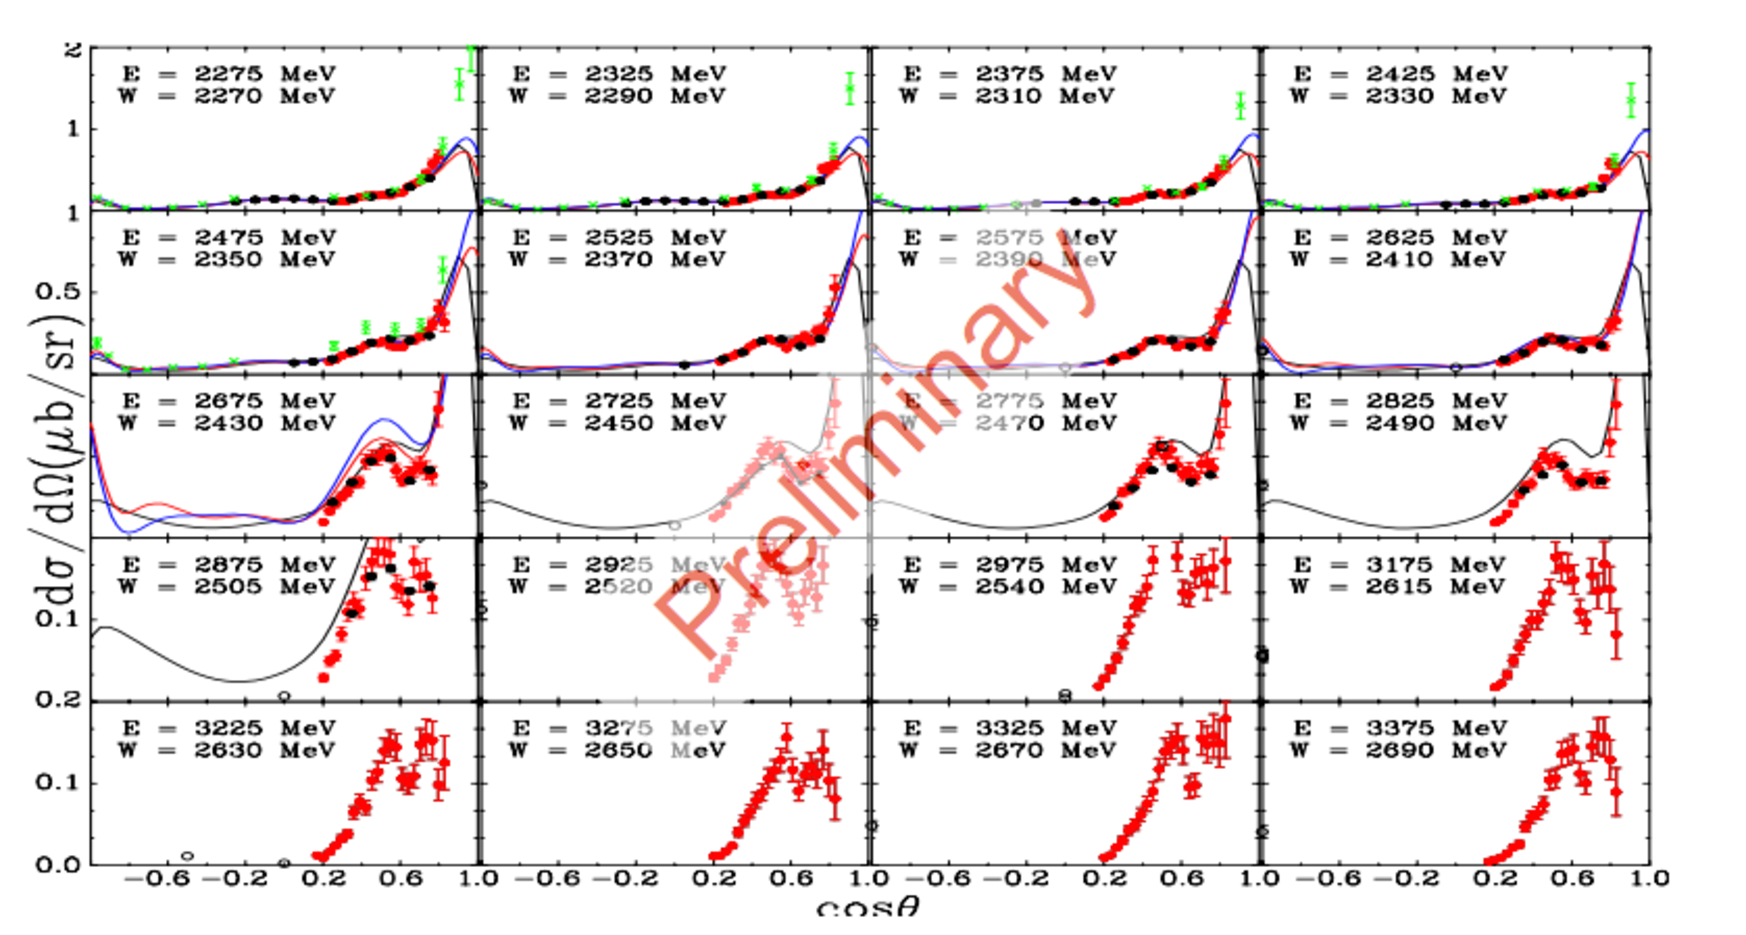
\includegraphics[width=225 pt, height = 160 pt]{figures/pi0_xsectionII.pdf}
		%\caption{figure in here}{box diagram}
		\caption{Left: $M_x^2 (p)$ vs. $M_E(pe^+e^-)$. The horizontal red dashed-dotted line depicts the 75 MeV cut used in this analysis. The vertical red dashed-dotted line depicts the boundary of single $\pi^0$ to $\pi^{+}\pi^{-}$ production. Right: Final $M_x^2(p)$ data used in analysis. The horizontal red dashed-dotted line depicts the threshold of $\pi^{+}\pi^{-}$ production.}{}
		\label{fig:pi0II}
	\end{minipage}
\end{figure}
\begin{figure}[h!]
	\centering
	\begin{minipage}{.50\textwidth}
		\centering
		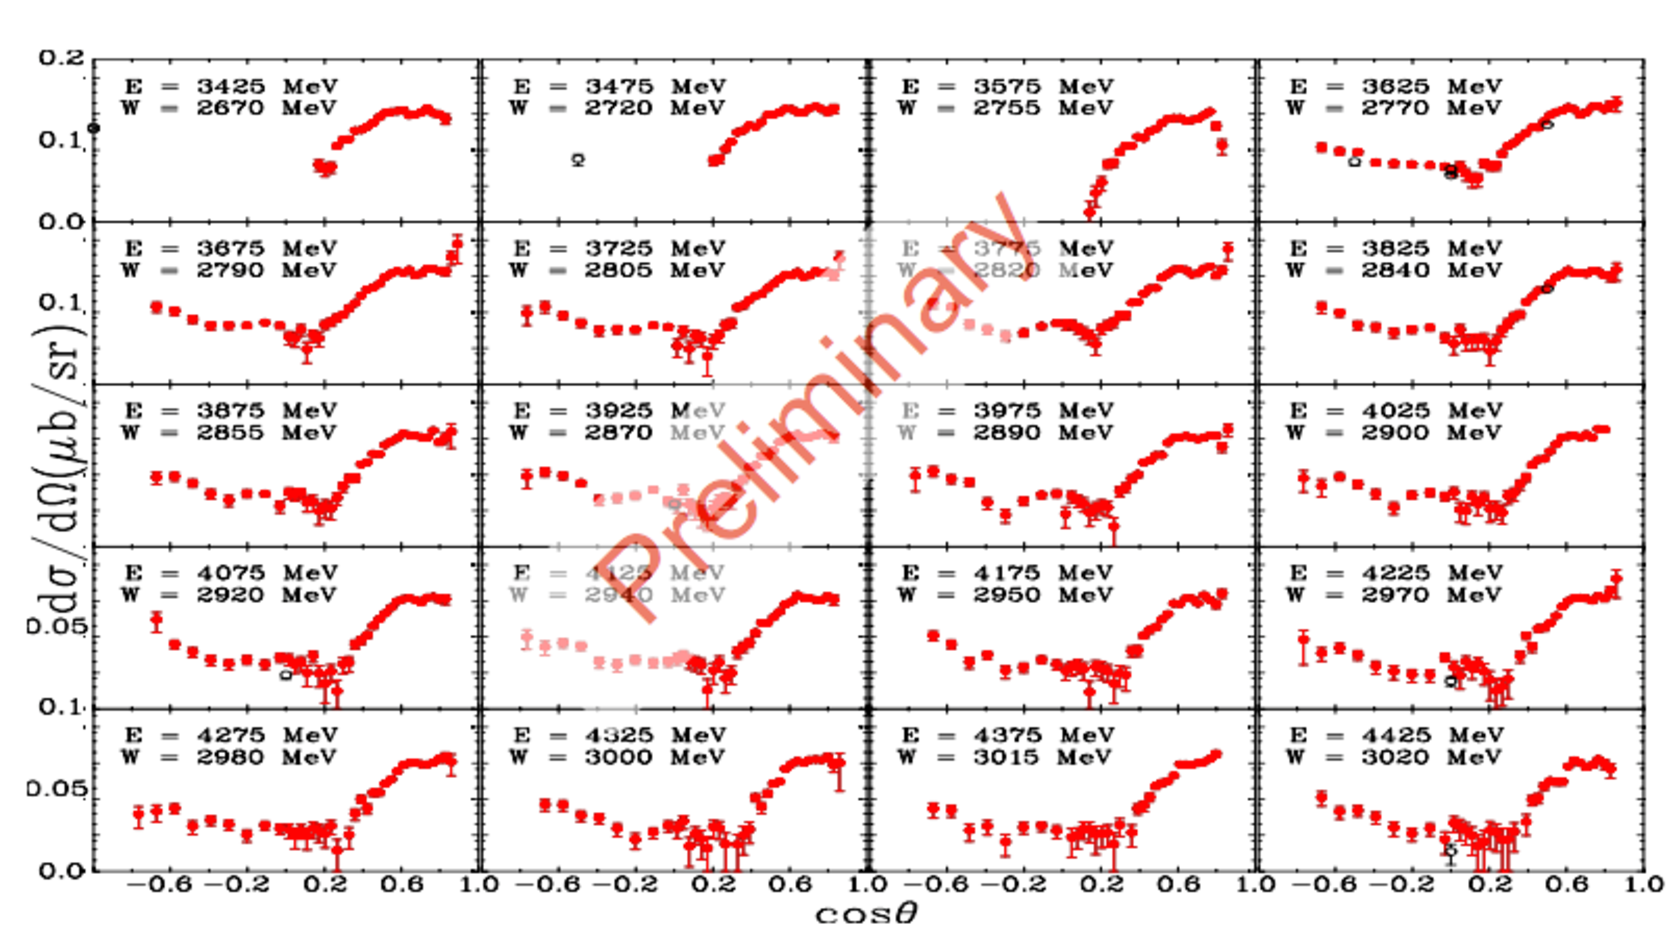
\includegraphics[width=225 pt, height = 160 pt]{figures/pi0_xsectionIII.pdf}
		\caption{}{}
		\label{fig:pi0III}
	\end{minipage}%
	\centering
	\begin{minipage}{.50\textwidth}
		\centering
		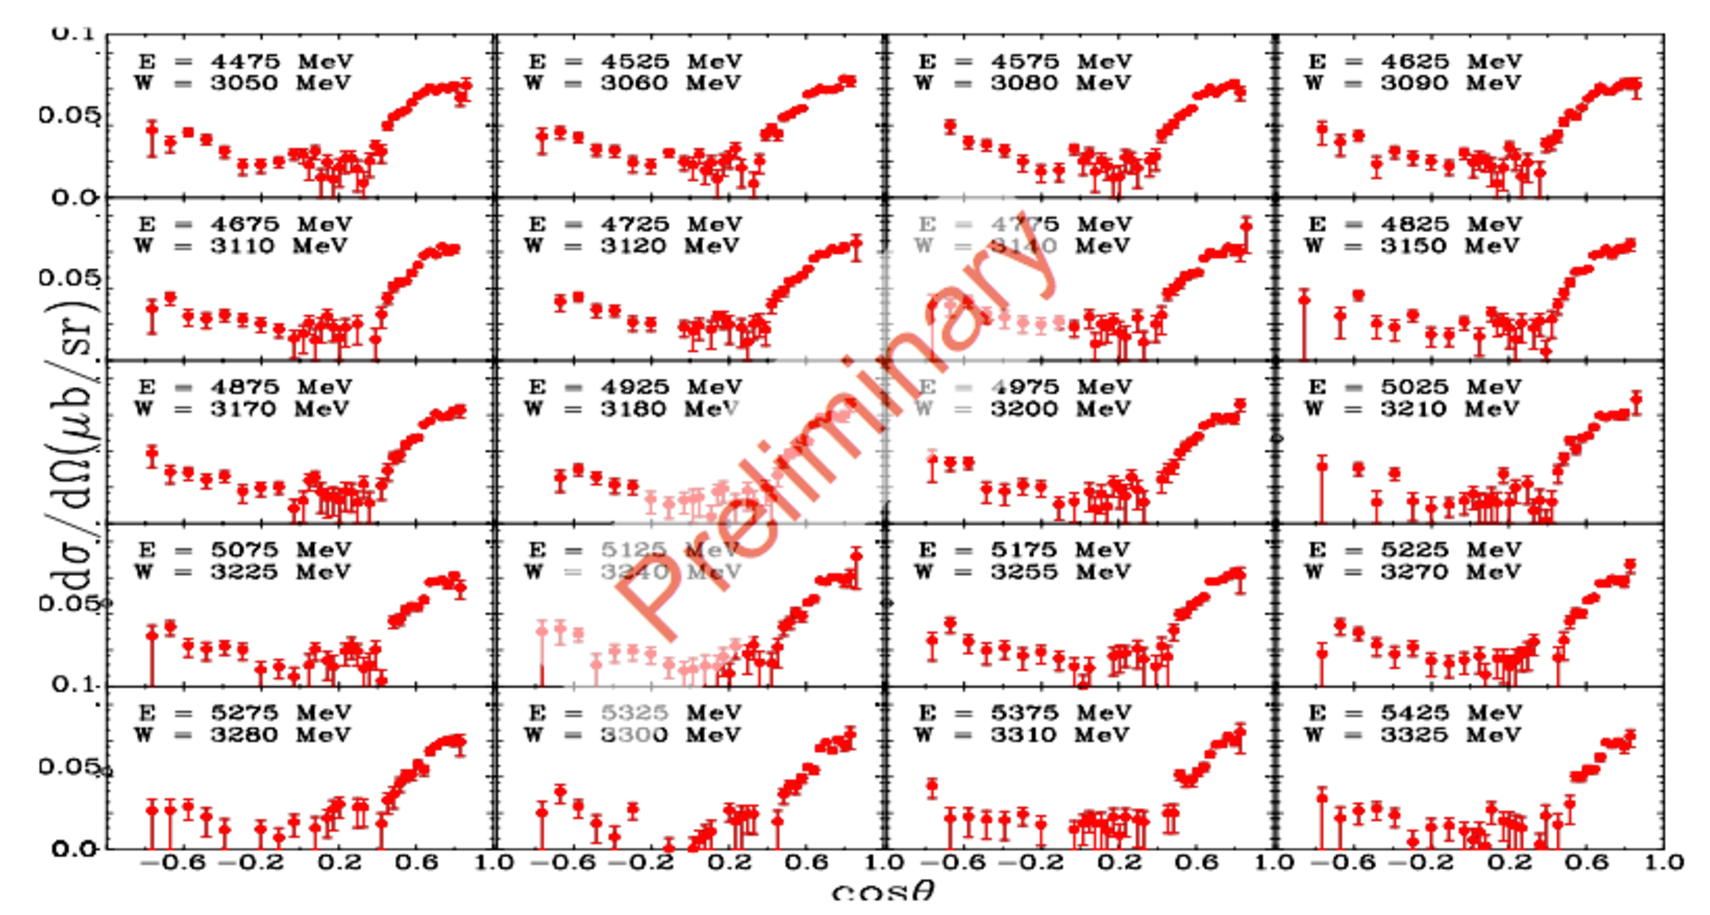
\includegraphics[width=225 pt, height = 155 pt]{figures/pi0_xsectionIV.pdf}
		%\caption{figure in here}{box diagram}
		\caption{Left: $M_x^2 (p)$ vs. $M_E(pe^+e^-)$. The horizontal red dashed-dotted line depicts the 75 MeV cut used in this analysis. The vertical red dashed-dotted line depicts the boundary of single $\pi^0$ to $\pi^{+}\pi^{-}$ production. Right: Final $M_x^2(p)$ data used in analysis. The horizontal red dashed-dotted line depicts the threshold of $\pi^{+}\pi^{-}$ production.}{}
		\label{fig:pi0IV}
	\end{minipage}
\end{figure}
\section{Comparison to Regge Model}
\begin{figure}[h]
	\centerline{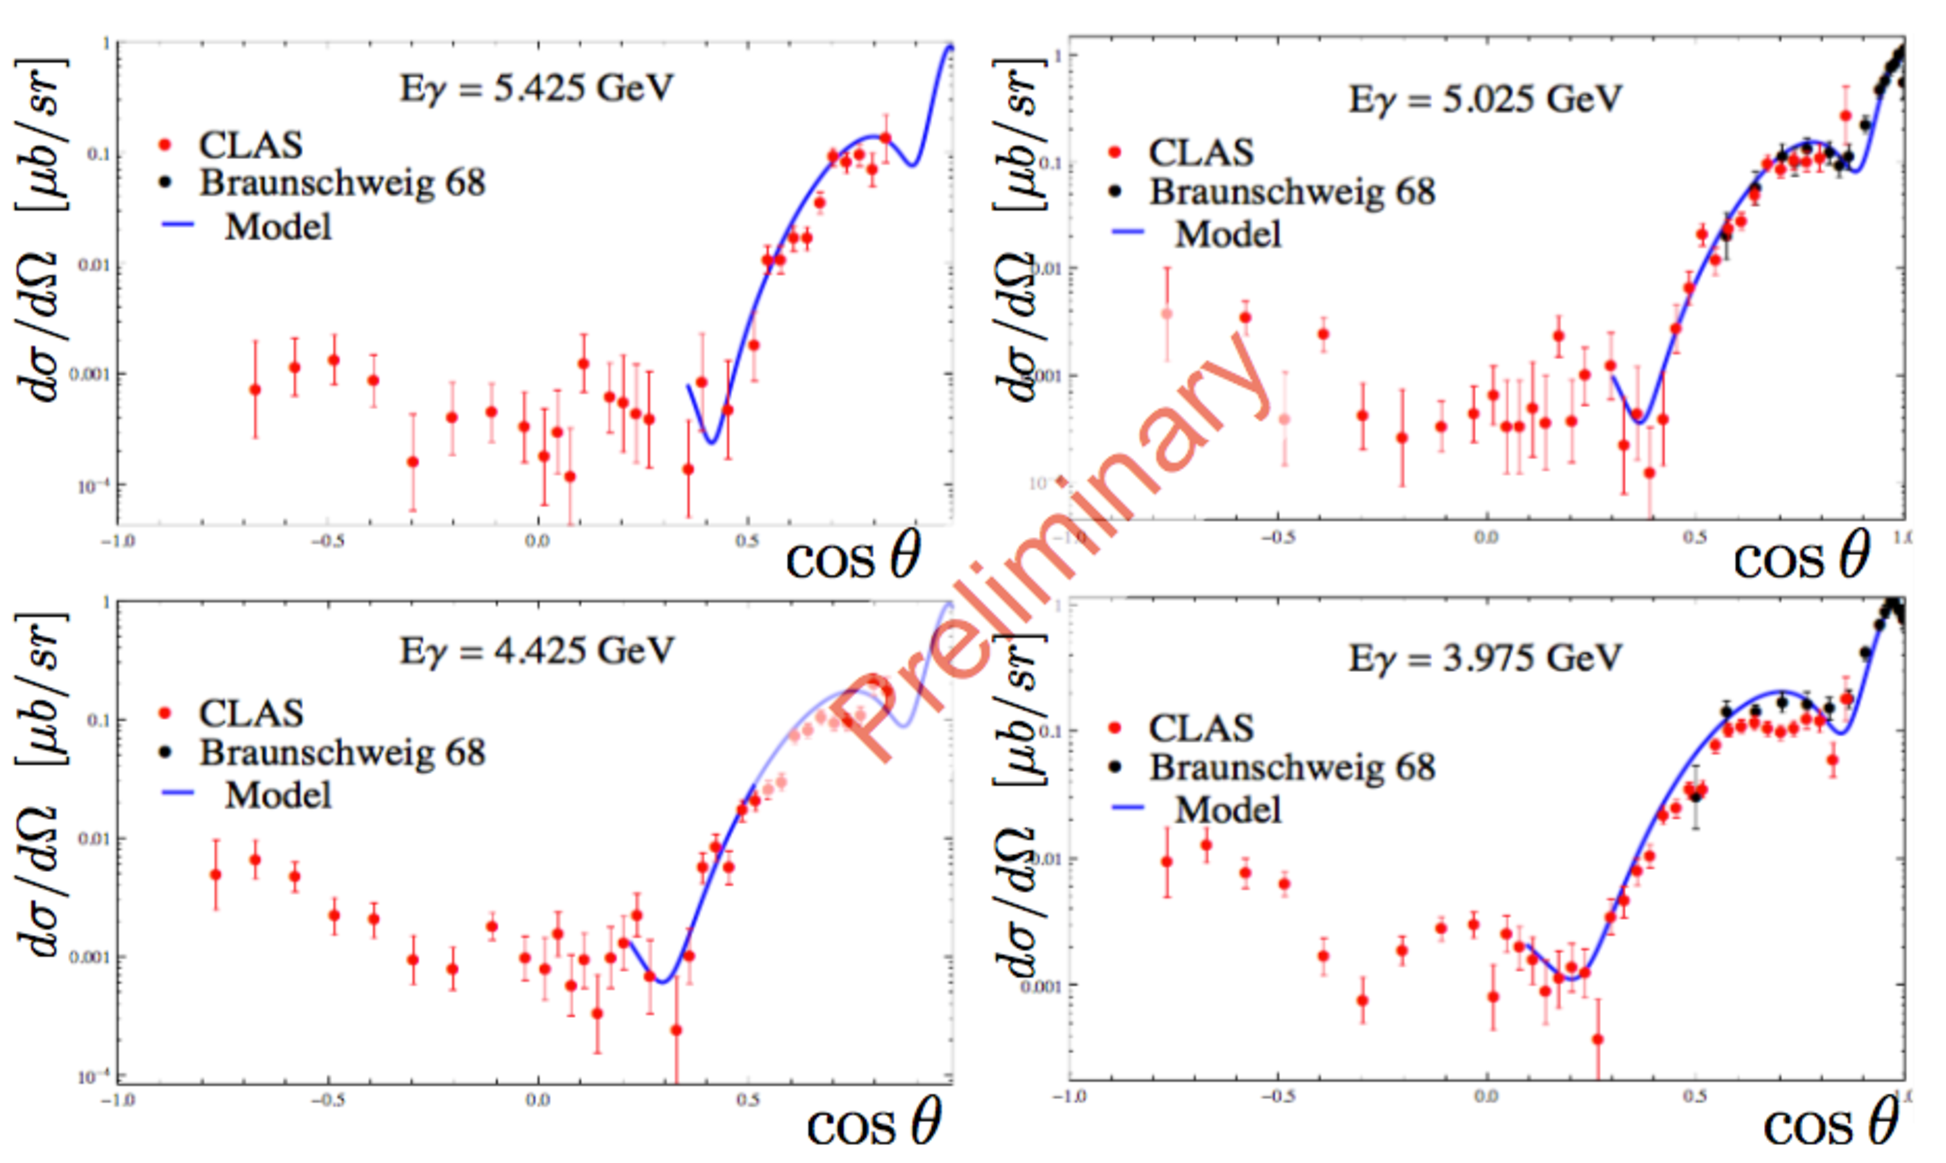
\includegraphics[width=225 pt]{figures/pi0_regge.pdf}}
	\caption{Comparison with Regge model. Caption embedded. }
	\label{fig:pi0_regge}
\end{figure}
\section{$s^7$ Scaling}
\begin{figure}[h]
	\centerline{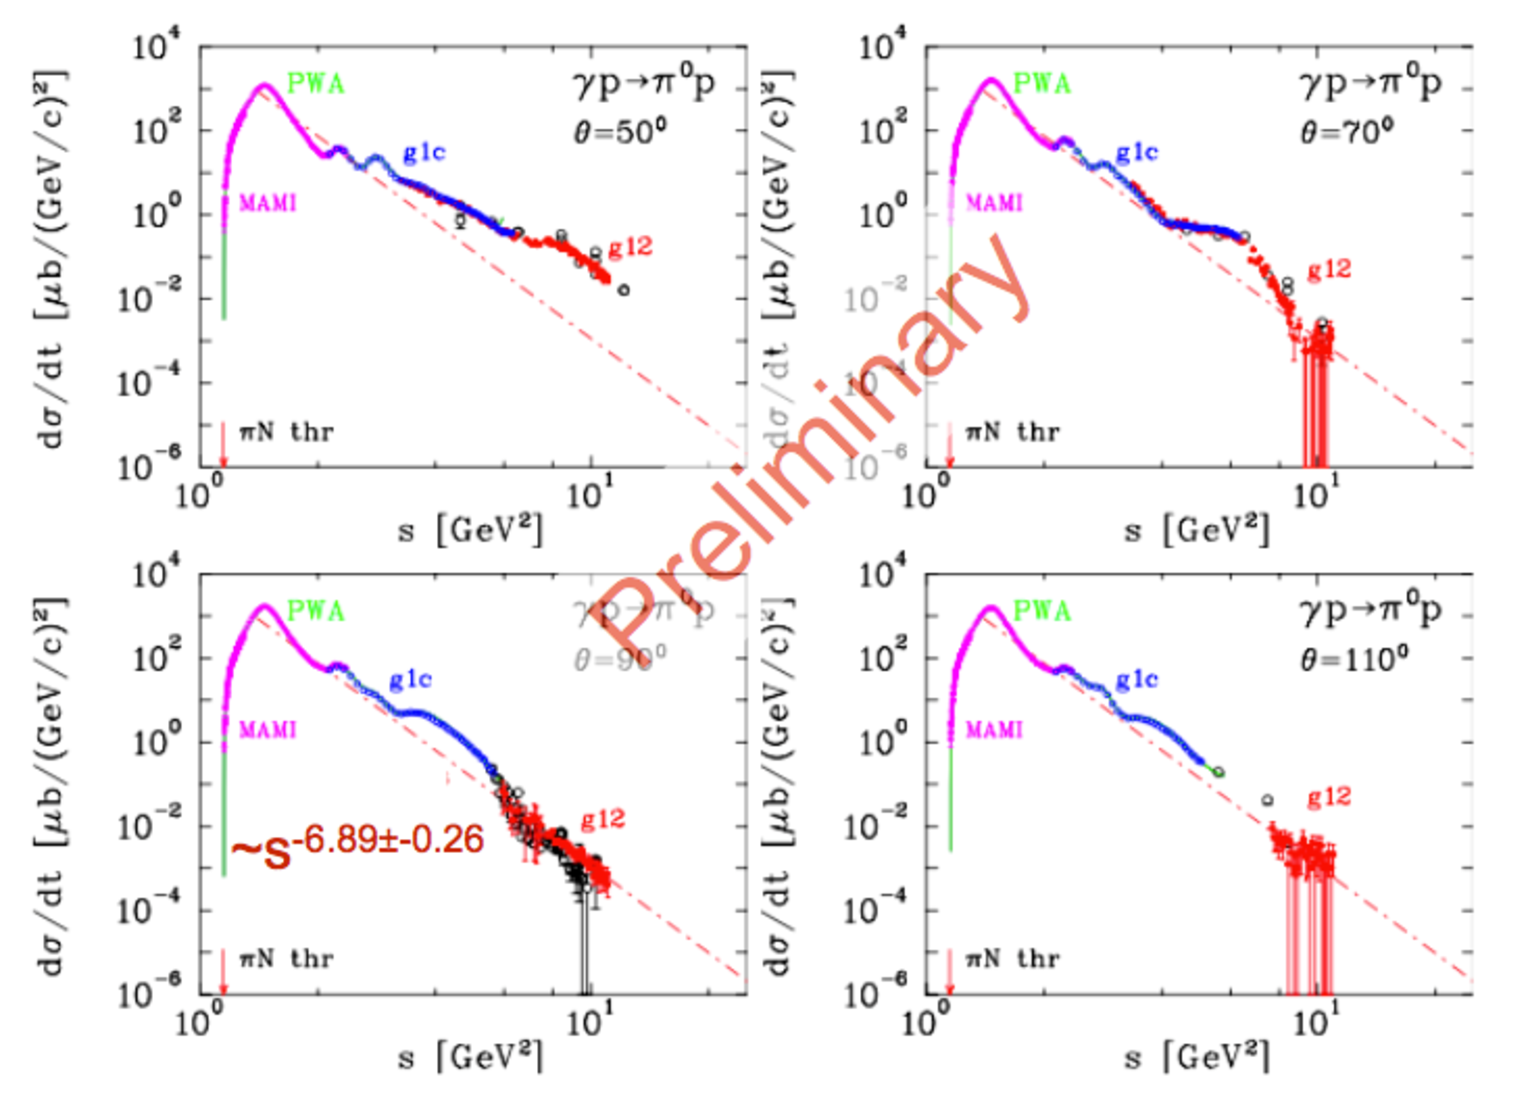
\includegraphics[width=225 pt]{figures/pi0_scaling.pdf}}
	\caption{Comparison with scaling rule. }
	\label{fig:pi0_scaling}
\end{figure}
\subsection{HALL C at Jlab12 Outlook}
\begin{figure}[h]
	\centerline{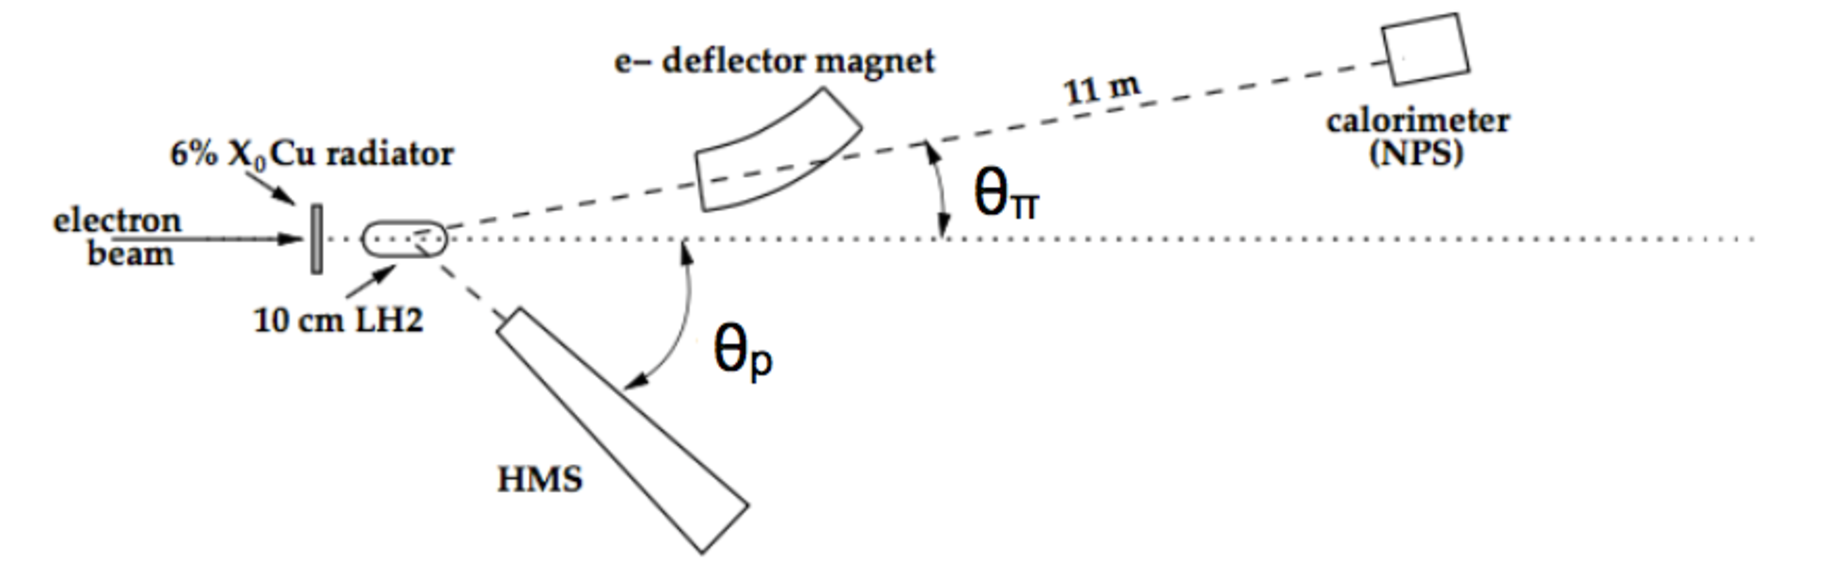
\includegraphics[width=225 pt]{figures/HALLC12.pdf}}
	\caption{Comparison with scaling rule. }
	\label{fig:hallc12}
\end{figure}
\begin{figure}[h]
	\centerline{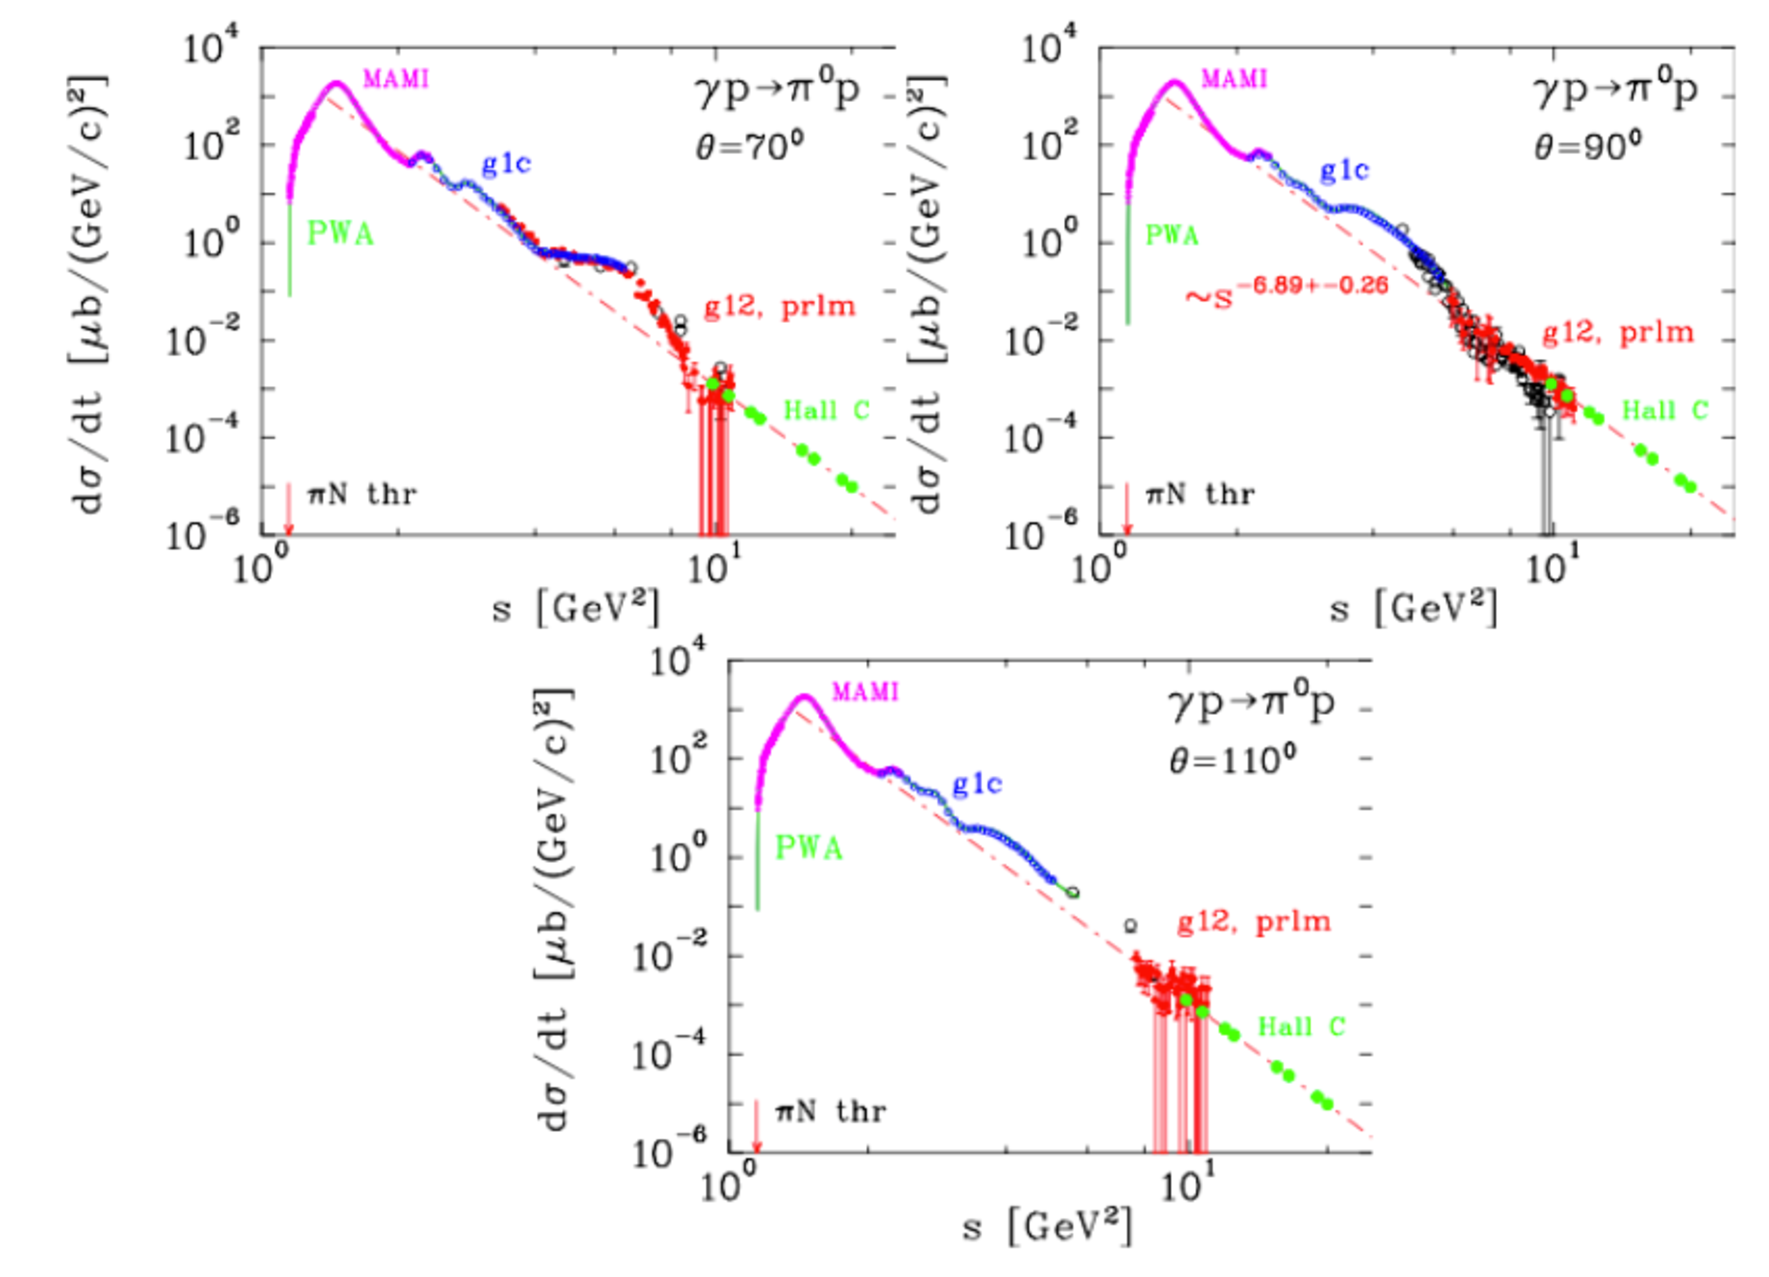
\includegraphics[width=225 pt]{figures/HallC_projected.pdf}}
	\caption{Comparison with scaling rule. }
	\label{fig:pi0_projected}
\end{figure}
% Acknowledgement
% References

\nocite{*}
\bibliographystyle{aipnum-cp}%
\bibliography{PI0}%


\end{document}
